\documentclass[10pt]{article}
\usepackage[polish]{babel}
\usepackage[utf8]{inputenc}
\usepackage[T1]{fontenc}
\usepackage{amsmath}
\usepackage{amsfonts}
\usepackage{amssymb}
\usepackage[version=4]{mhchem}
\usepackage{stmaryrd}
\usepackage{graphicx}
\usepackage[export]{adjustbox}
\graphicspath{ {./images/} }

\title{KLASY PO SZKOLE PODSTAWOWEJ }

\author{}
\date{}


\begin{document}
\maketitle
\begin{enumerate}
  \item Pewien trójkąt ma boki o długościach: \(x, x+1, x+2\) gdzie \(x>3\). Wysokość poprowadzona na bok o długości \(x+1\) dzieli ten bok na dwa odcinki. Wykaż, że jeden z tych odcinków jest o 4 dłuższy od drugiego.\\
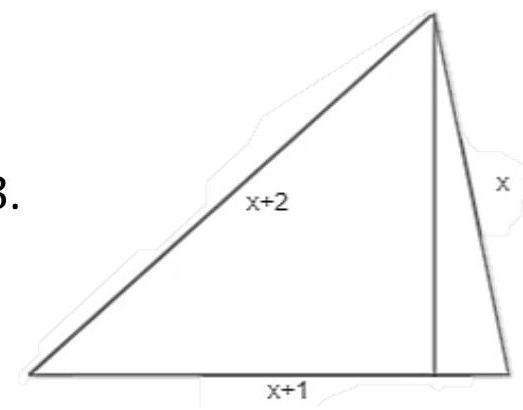
\includegraphics[max width=\textwidth, center]{2024_11_21_4f01d8a613fbbdc215e5g-1}
  \item Pewna klasa liczy 20 uczniów, wpisanych do dziennika pod numerami od 1 do 20. Ustaw uczniów w pary tak, by suma numerów uczniów każdej pary była podzielna przez 6.
  \item Niech \(x y z=1, a=x+\frac{1}{x}, b=y+\frac{1}{y}, c=z+\frac{1}{z}\). Wykaż, że jeżeli \(a b c\) jest liczbą całkowitą, to \(a^{2}+b^{2}+c^{2}\) też jest liczbą całkowitą.
\end{enumerate}

\section*{KLASY PO GIMNAZJUM}
\begin{enumerate}
  \item Dany jest kwadrat \(A B C D\). Na bokach BC i CD wybrano odpowiednio punkty E i F tak, że \(\mathrm{BE}+\mathrm{DF}=\mathrm{EF}\). Udowodnij, że kąt EAF ma \(45^{\circ}\).
  \item W konfiguracji z zadania 1 udowodnij, że środek okręgu opisanego na trójkącie AEF leży na przekątnej AC danego kwadratu.
  \item W konfiguracji z zadania 1 punkt G jest rzutem prostokątnym punktu A na prostą EF, a punkty H oraz I są odpowiednio punktami wspólnymi przekątnej BD z odcinkami AE i AF. Udowodnij, że proste AG, El oraz FH przecinają się w jednym punkcie.\\
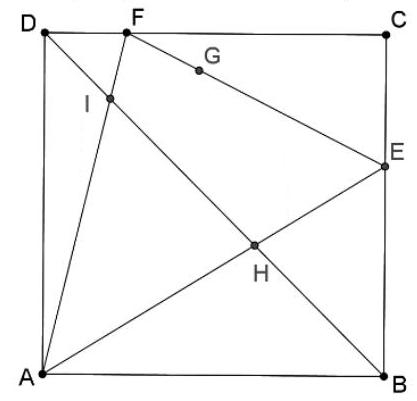
\includegraphics[max width=\textwidth, center]{2024_11_21_4f01d8a613fbbdc215e5g-1(1)}
\end{enumerate}

\end{document}